\begin{abstract}

Our analysis of the key-value activity generated by the ParSplice molecular
dynamics simulation demonstrates the need for more complex cache management
strategies. Baseline measurements show clear keyspace access patterns and hot
spots that offer significant opportunity for optimization. We use the data
management and policy engine from the Mantle system to dynamically explore a
variety of techniques, ranging from basic algorithms and heuristics to
statistical models, calculus, and machine learning. While Mantle was originally
designed for distributed file systems, we show how the collection of
abstractions effectively decomposes the problem into manageable policies for a
different domain and service.  Our exploration of this space results in a two
policy scheme that achieves 96\% efficiency while using only 7.6\% of the
memory resources required by the base case. 

\end{abstract}

\section{Introduction}

The fine-grained data annotation capabilities provided by key-value storage is
a natural match for many types of scientific simulation. Simulations relying on
a mesh-based decomposition of a physical region may result in millions or
billions of mesh cells. Each cell contains materials, pressures, temperatures
and other characteristics that are required to accurately simulate phenomena of
interest. In our target application, the
ParSplice~\cite{perez:jctc20150parsplice} molecular dynamics simulation, a
hierarchy of caches and a single persistent key-value store are used to store
both observed minima across a molecule's equation of motion (EOM) and the
hundreds or thousands of partial trajectories calculated each second during a
parallel job. Unfortunately, if we scale the system the IO to the storage
hierarchy will quickly saturate both the storage and bandwidth capacity of a
single node, so we need more effective data management techniques, such as
cache management or load balancing across a cluster.

\begin{figure}[t]
  \noindent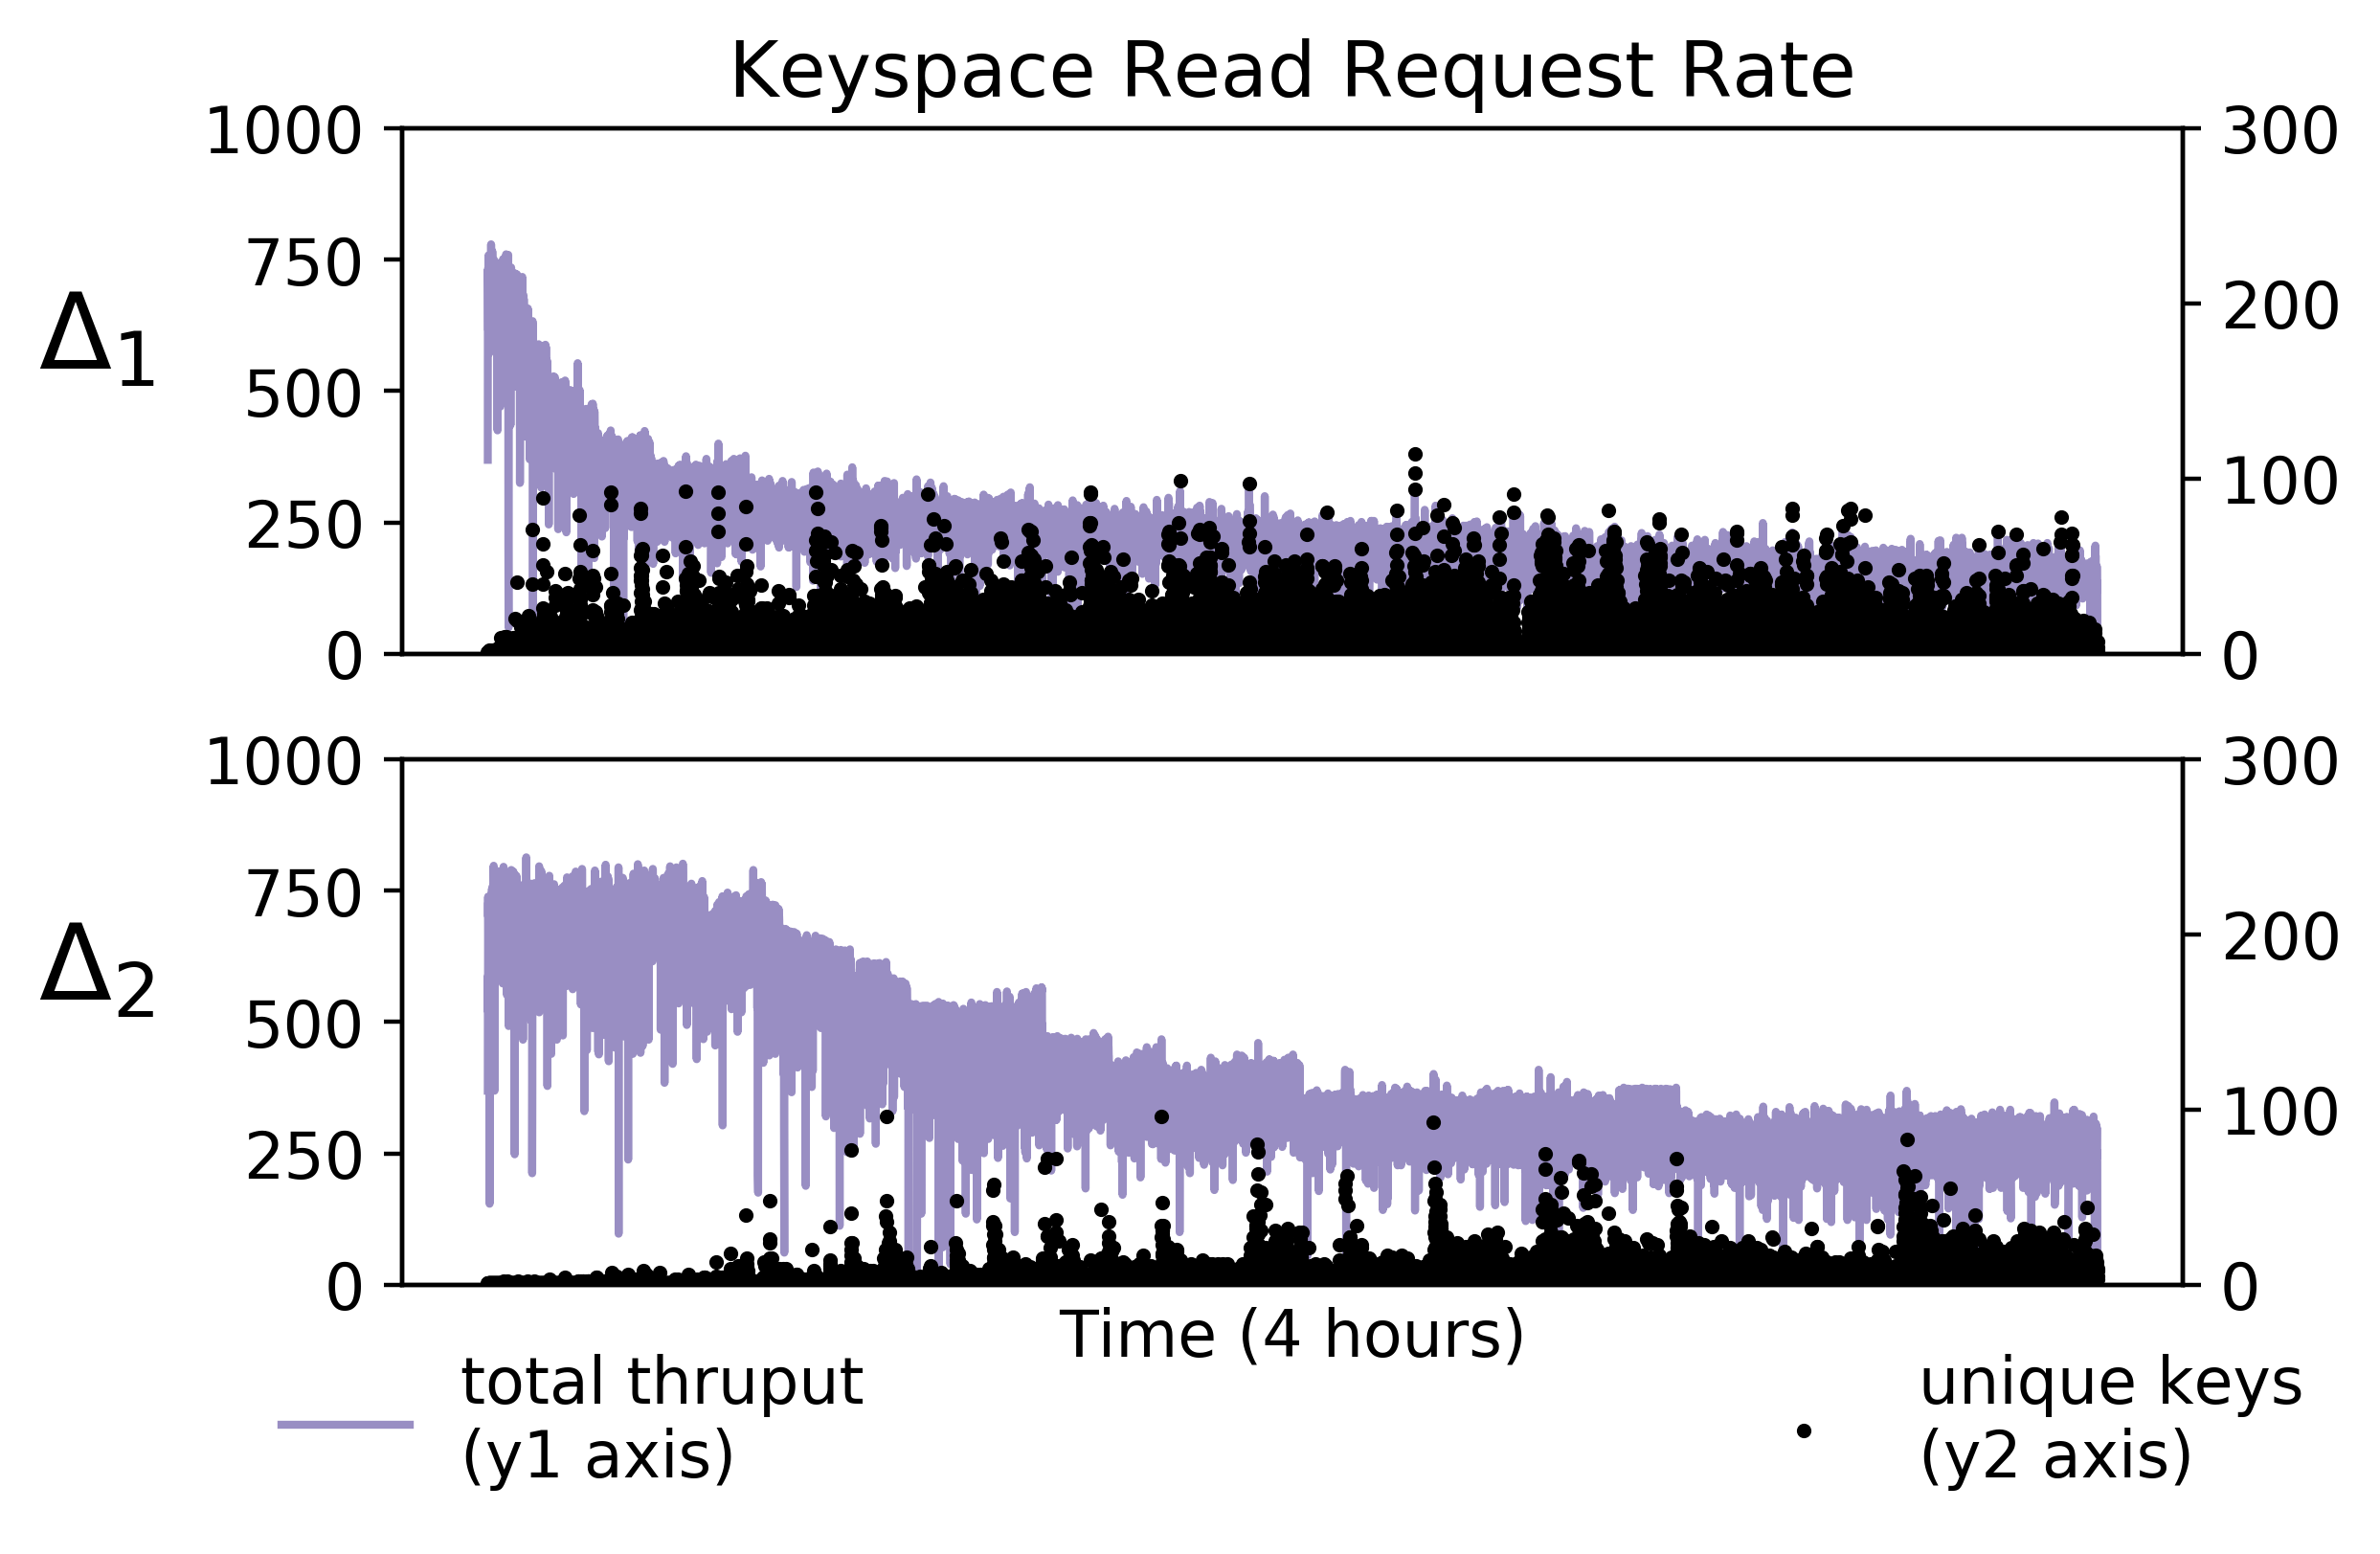
\includegraphics[width=0.5\textwidth]{figures/motivation-regimes.png}\\
  \caption{The keyspace activity for ParSplice using two different growth
rates.  The line shows the rate that EOM minima values are retrieved from the
key-value store (\(y1\) axis) and the points along the bottom show the number
of keys accessed in a 1 second sliding window (\(y2\) axis).
\label{fig:motivation-regimes}}
\end{figure}

In this paper, we design cache management policies for the ParSplice worker,
driven by a detailed analysis of the key-value accesses over the course of a
long running simulation across a variety of initial conditions.
Figure~\ref{fig:motivation-regimes} shows how ParSplice tasks read key-value
pairs from the worker's cache for two different initial conditions of
\(\Delta\), which is the rate that new atoms enter the simulation.  The line is
the read request rate (\(y1\) axis) and the dots along the bottom are the
number of unique keys accessed (\(y2\) axis).  This figure demonstrates that
small changes to \(\Delta\) can have a strong effect on the timing and
frequency with which new EOM minima are discovered and referenced.  The
ParSplice caches on each node are trimmed when memory pressure reaches a
threshold but the number of unique keys accessed in
Figure~\ref{fig:motivation-regimes} suggests that a small cache of EOM minima
should be sufficient. 

% What is Mantle
We use the data management language and policy engine from the Mantle
paper~\cite{sevilla:sc15-mantle} to dynamically explore the effects of
different cache management strategies for the changing key-value workloads
generated by ParSplice.  Mantle was originally touted as a programmable file
system metadata load balancer, but we realize now that the collection of
abstractions designed for file systems was a control plane that improved
metadata access. So in this paper we refer to Mantle as a policy engine that
injects policies written in our data management language directly into a
running service and show how this approach is useful for reasoning about and
designing different cache management strategies in ParSplice.  By service, we
mean a system that manages data and responds requests, such as a file system or
key-value store.  Developers write policies for ``when" they want data moved
and ``how much" of the data to move, then the framework executes these policies
whenever a decision needs to be made.  These abstraction help developers
unfamiliar with the domain quickly reason about, develop, and deploy new
policies that control temporal and spatial locality. We show that Mantle:

\begin{itemize}

  \item decomposes cache management into independent policies that can be
  dynamically changed, making the problem more manageable and facilitating rapid
  development. Changing the policy in use is critical in applications such as
  ParSplice that have alternating stable and chaotic keyspace access patterns
  over the course of a long-running simulation.  

  \item can be used to quickly deploy a variety of cache management strategies,
  ranging from basic algorithms and heuristics to statistical models and machine
  learning.

  \item has useful primitives that, while designed for file system metadata
  load balancing, turn out to also be effective for cache management. This
  finding shows how the policy engine generalizes to different domains and
  enables control of policies by machines instead of administrators.

\end{itemize}

% this gives us many policies that are effective across disciplines
% - reuse: eases burden of writing policies
% - autonomic: lays groundwork for an adaptable policy that mixes/matches policies
% FUTURE WORK

This last contribution is explored in
Sections~\S\ref{sec:cache-management-using-system-archiecture-knowledge}
and~\S\ref{sec:cache-management-using-domain-specific-knowledge}, where we try
a range of policies from different disciplines; but more importantly, in
Section~\S\ref{sec:relation-to-load-balancing}, we conclude that the collection
of policies we designed for ParSplice's cache management are very similar to
the policies used to load balance metadata in the Ceph file system (CephFS)
suggesting that there is potential for automatically adapting and generating
policies dynamically. 

%Manageable: abstracts away complexities of the system (pass around to others,
%use different strategies) 

